\documentclass{article}
\usepackage[utf8]{vietnam}
\usepackage{graphicx}
% \usepackage{hyperref}

%%%%%%%%%%%%%%%%%%%%%%%%%%%%%%%%%%%%%%%%%%%%%%%%%%%%%%%
\begin{document}
% \tableofcontents
% \newpage
%%%%%%%%%%%%%%%%%%%%%%%%%%%%%%%%%%%%%%%%%%%%%%%%%%%%%%%
\section{Tuần 1}



\subsection{Video 1}

\subsubsection{Hướng dẫn}

% \paragraph{Hướng dẫn sắp xếp dữ liệu}
% \subparagraph{Hướng dẫn sắp xếp dữ liệu theo 1 tiêu chí}
% \begin{figure}[h]
%     \centering
%     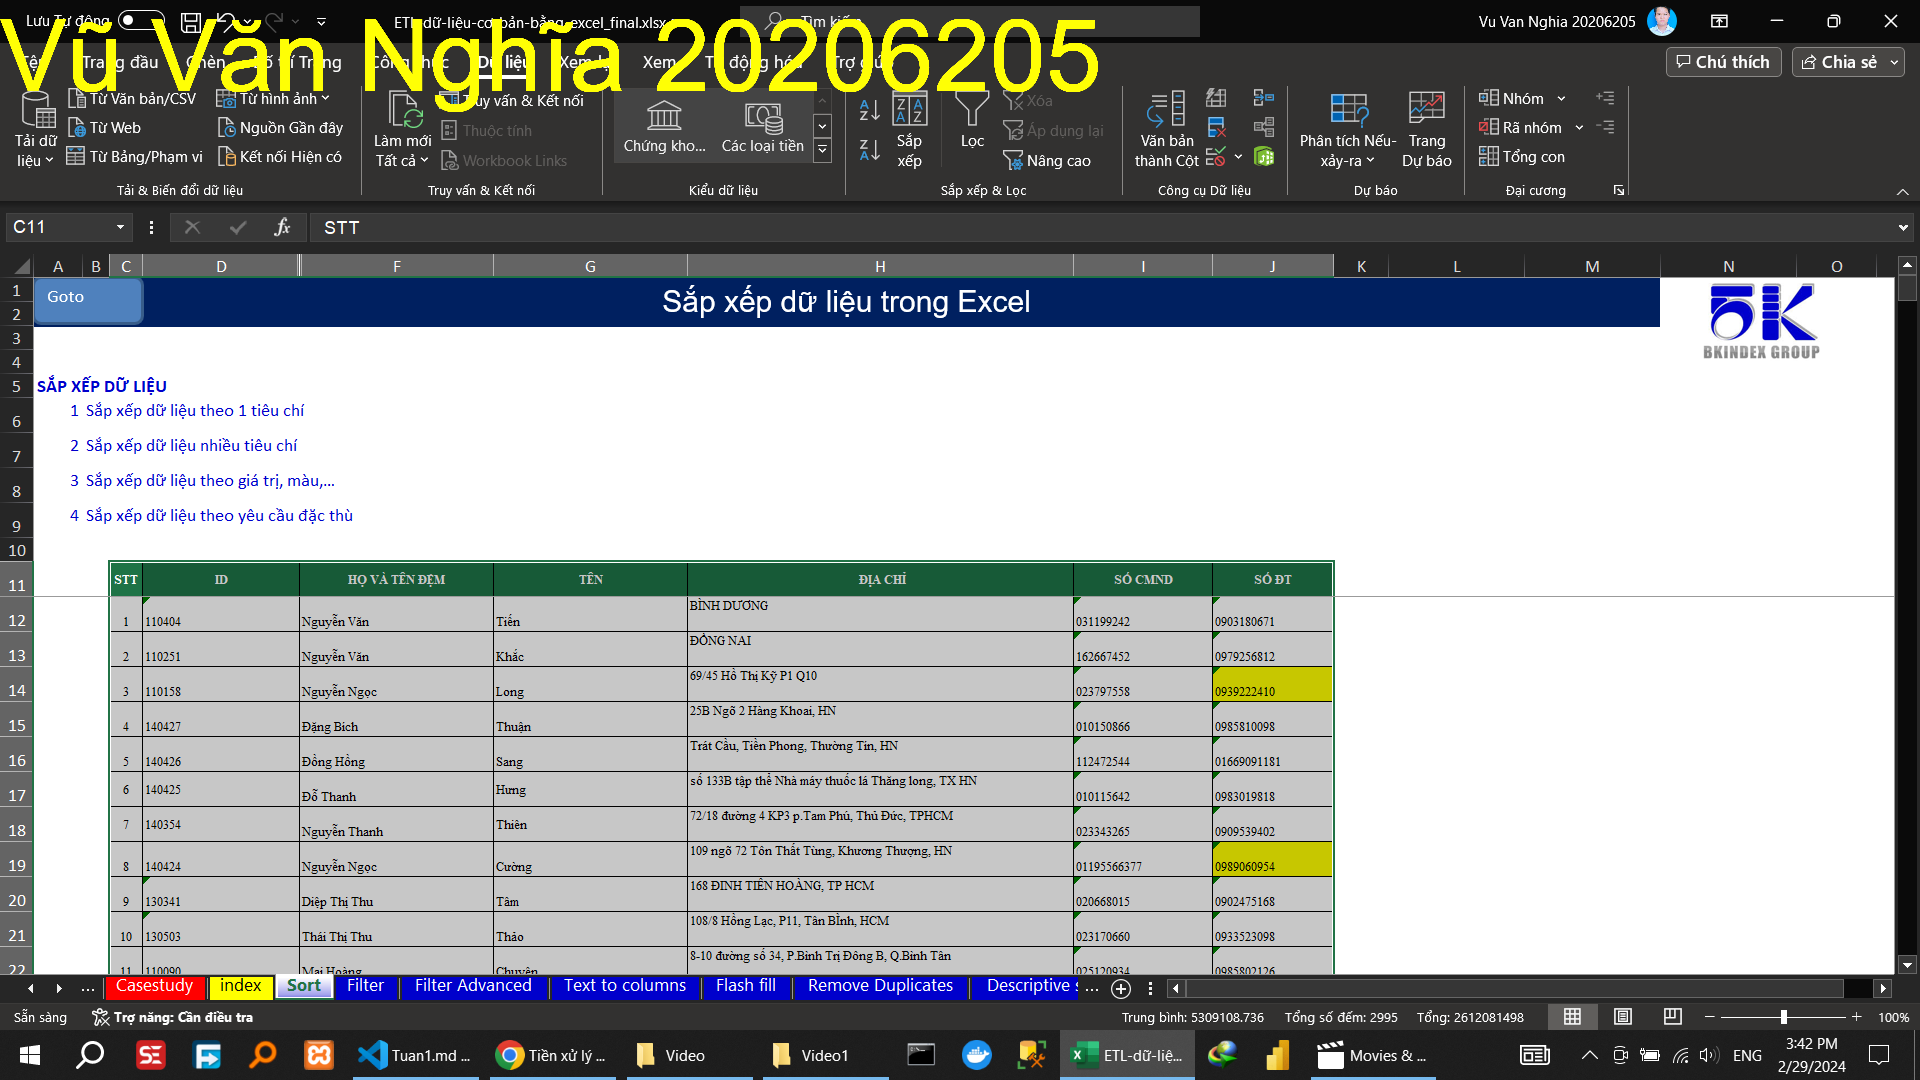
\includegraphics[scale = 0.15]{Video1/HuongDan/1.png}
%     \caption{Hướng dẫn sắp xếp dữ liệu theo 1 tiêu chí là số thứ tự}
% \end{figure}
% \subparagraph{Hướng dẫn sắp xếp dữ liệu theo nhiều tiêu chí}
% \begin{figure}[h]
%     \centering
%     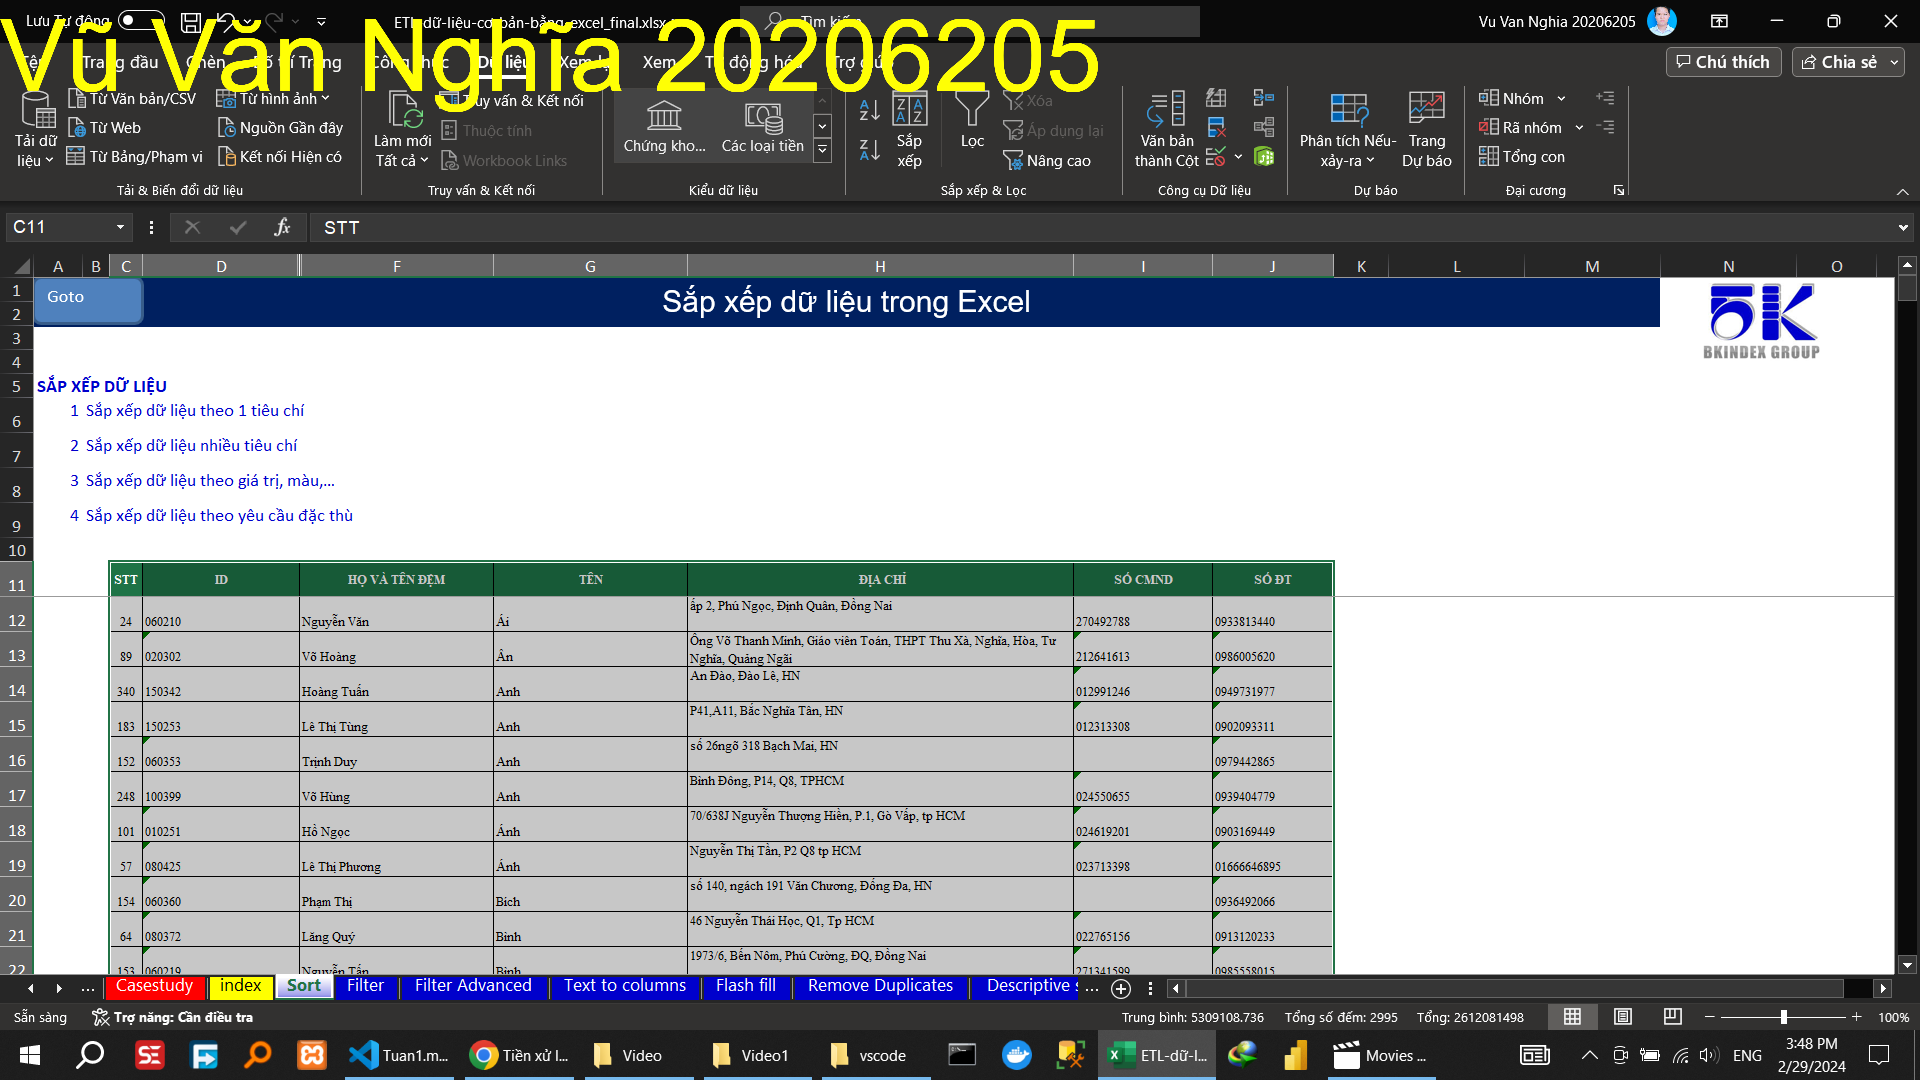
\includegraphics[scale = 0.15]{Video1/HuongDan/2.png}
%     \caption{Hướng dẫn sắp xếp dữ liệu theo  nhiều tiêu chí họ và tên đệm}
% \end{figure}
% \subparagraph{Hướng dẫn sắp xếp dữ liệu theo giá trị, màu,\dots}
% \begin{figure}[h]
%     \centering
%     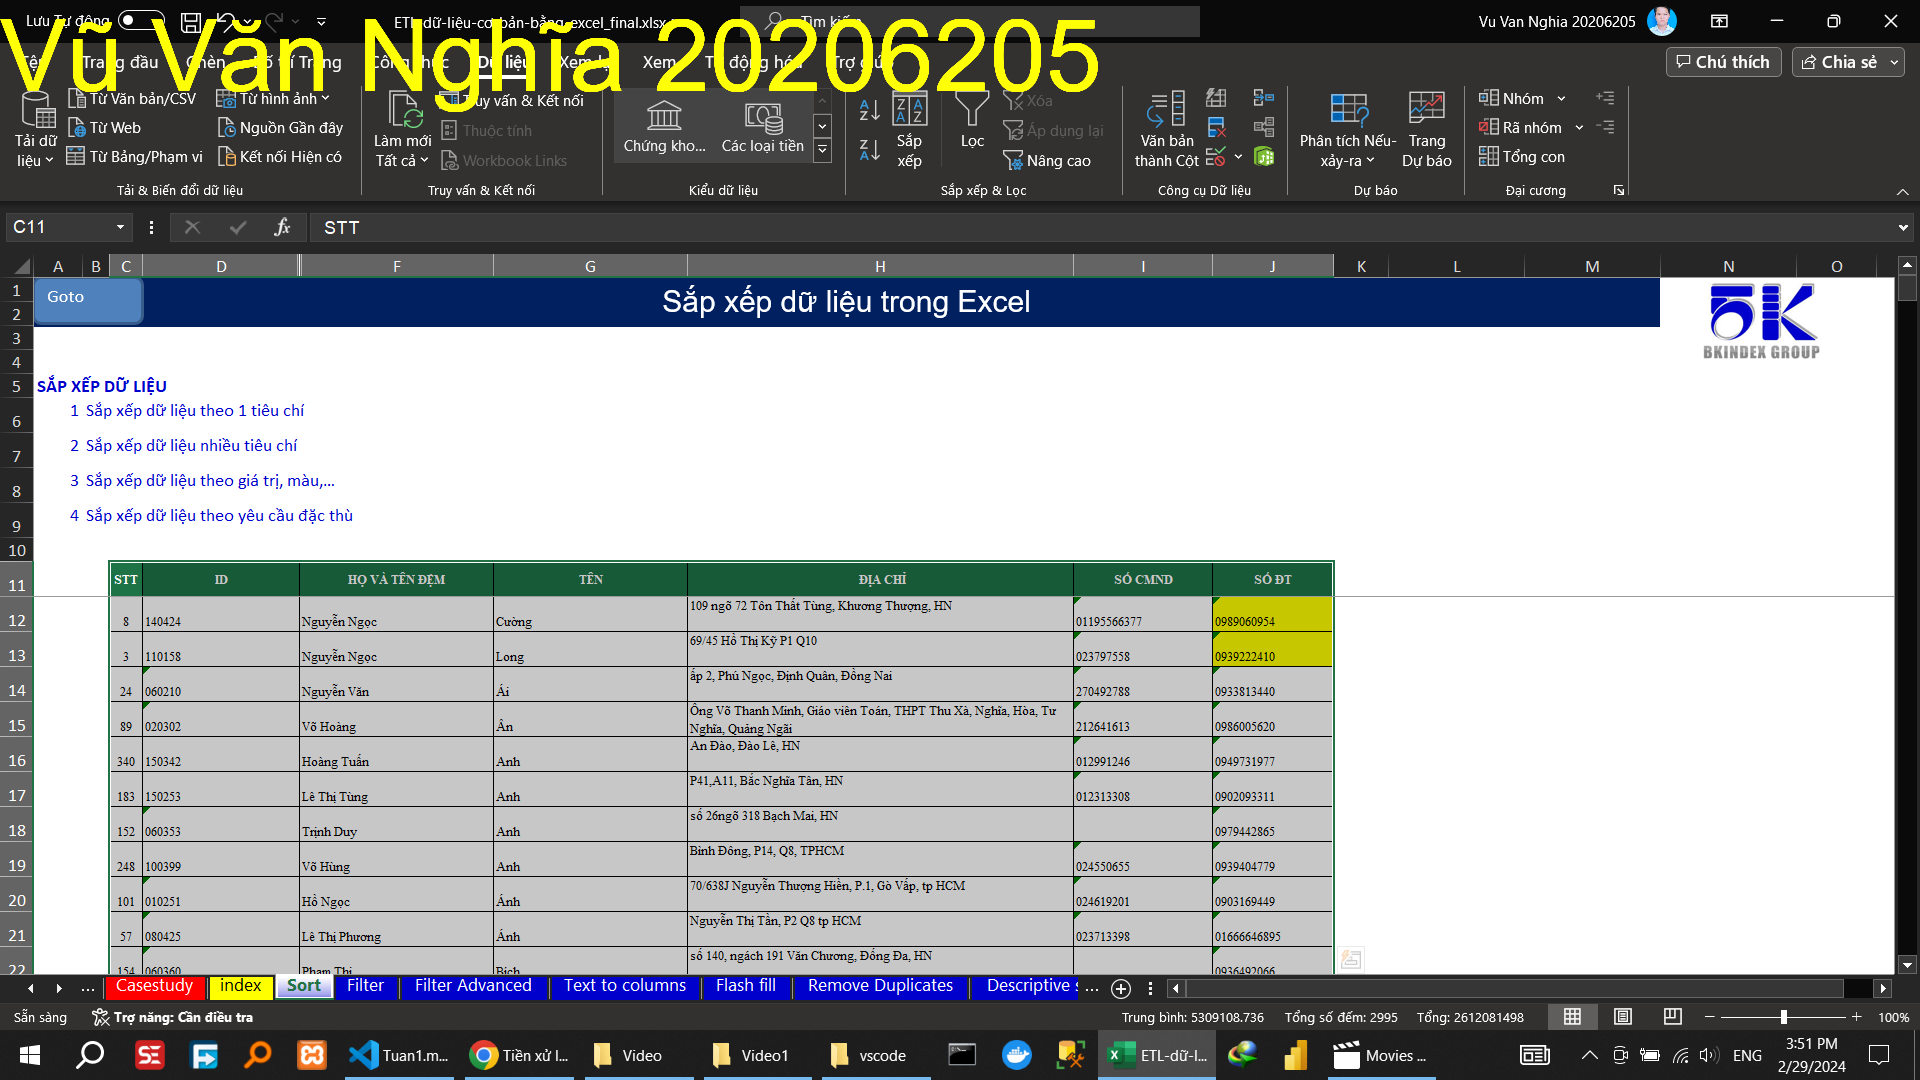
\includegraphics[scale = 0.15]{Video1/HuongDan/3.png}
%     \caption{Hướng dẫn sắp xếp dữ liệu theo  giá trị, màu,\dots của số điện thoại}
% \end{figure}




% \paragraph{Hướng dẫn lọc dữ liệu}
% \subparagraph{Hướng dẫn lọc dữ liệu theo 1 tiêu chí}
% \begin{figure}[h]
%     \centering
%     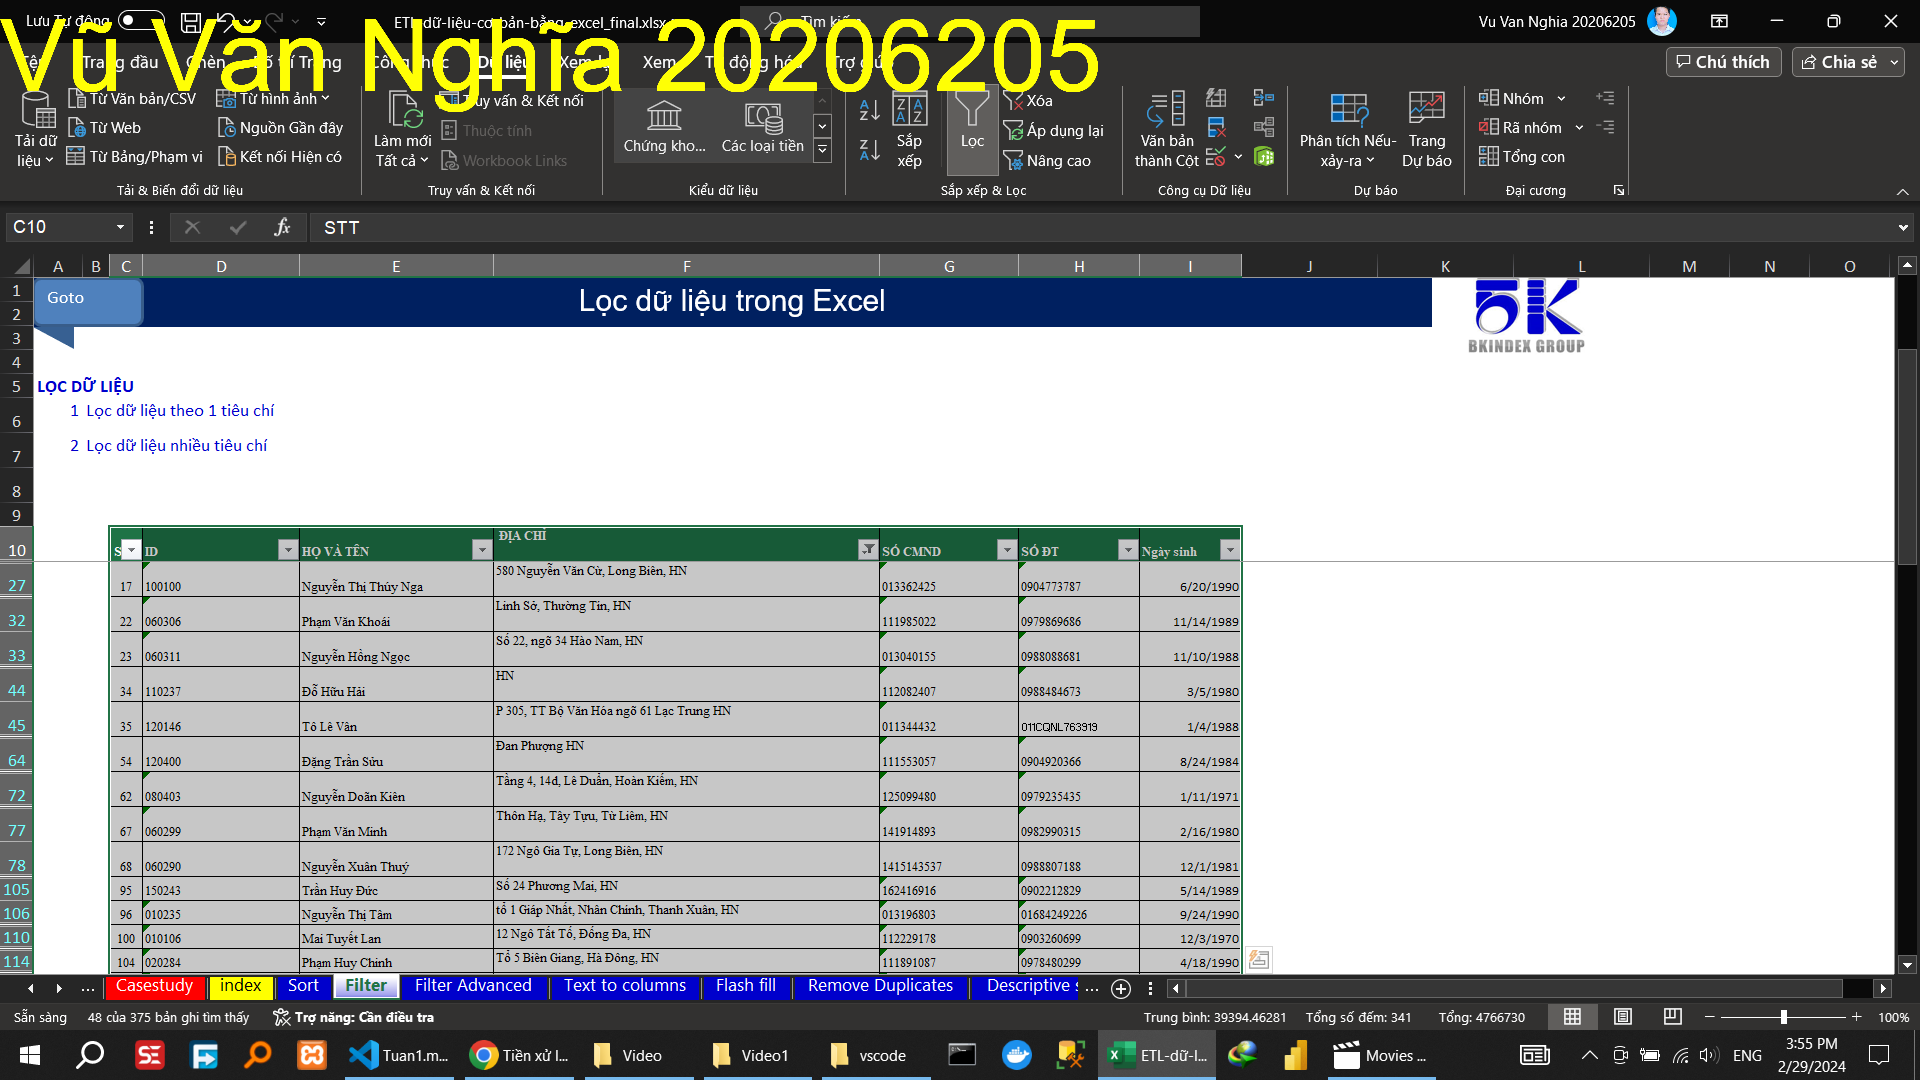
\includegraphics[scale = 0.15]{Video1/HuongDan/4.png}
%     \caption{Hướng dẫn lọc dữ liệu theo 1 tiêu chí là địa chỉ HN}
% \end{figure}
% \subparagraph{Hướng dẫn lọc dữ liệu theo nhiều tiêu chí}
% \begin{figure}[h]
%     \centering
%     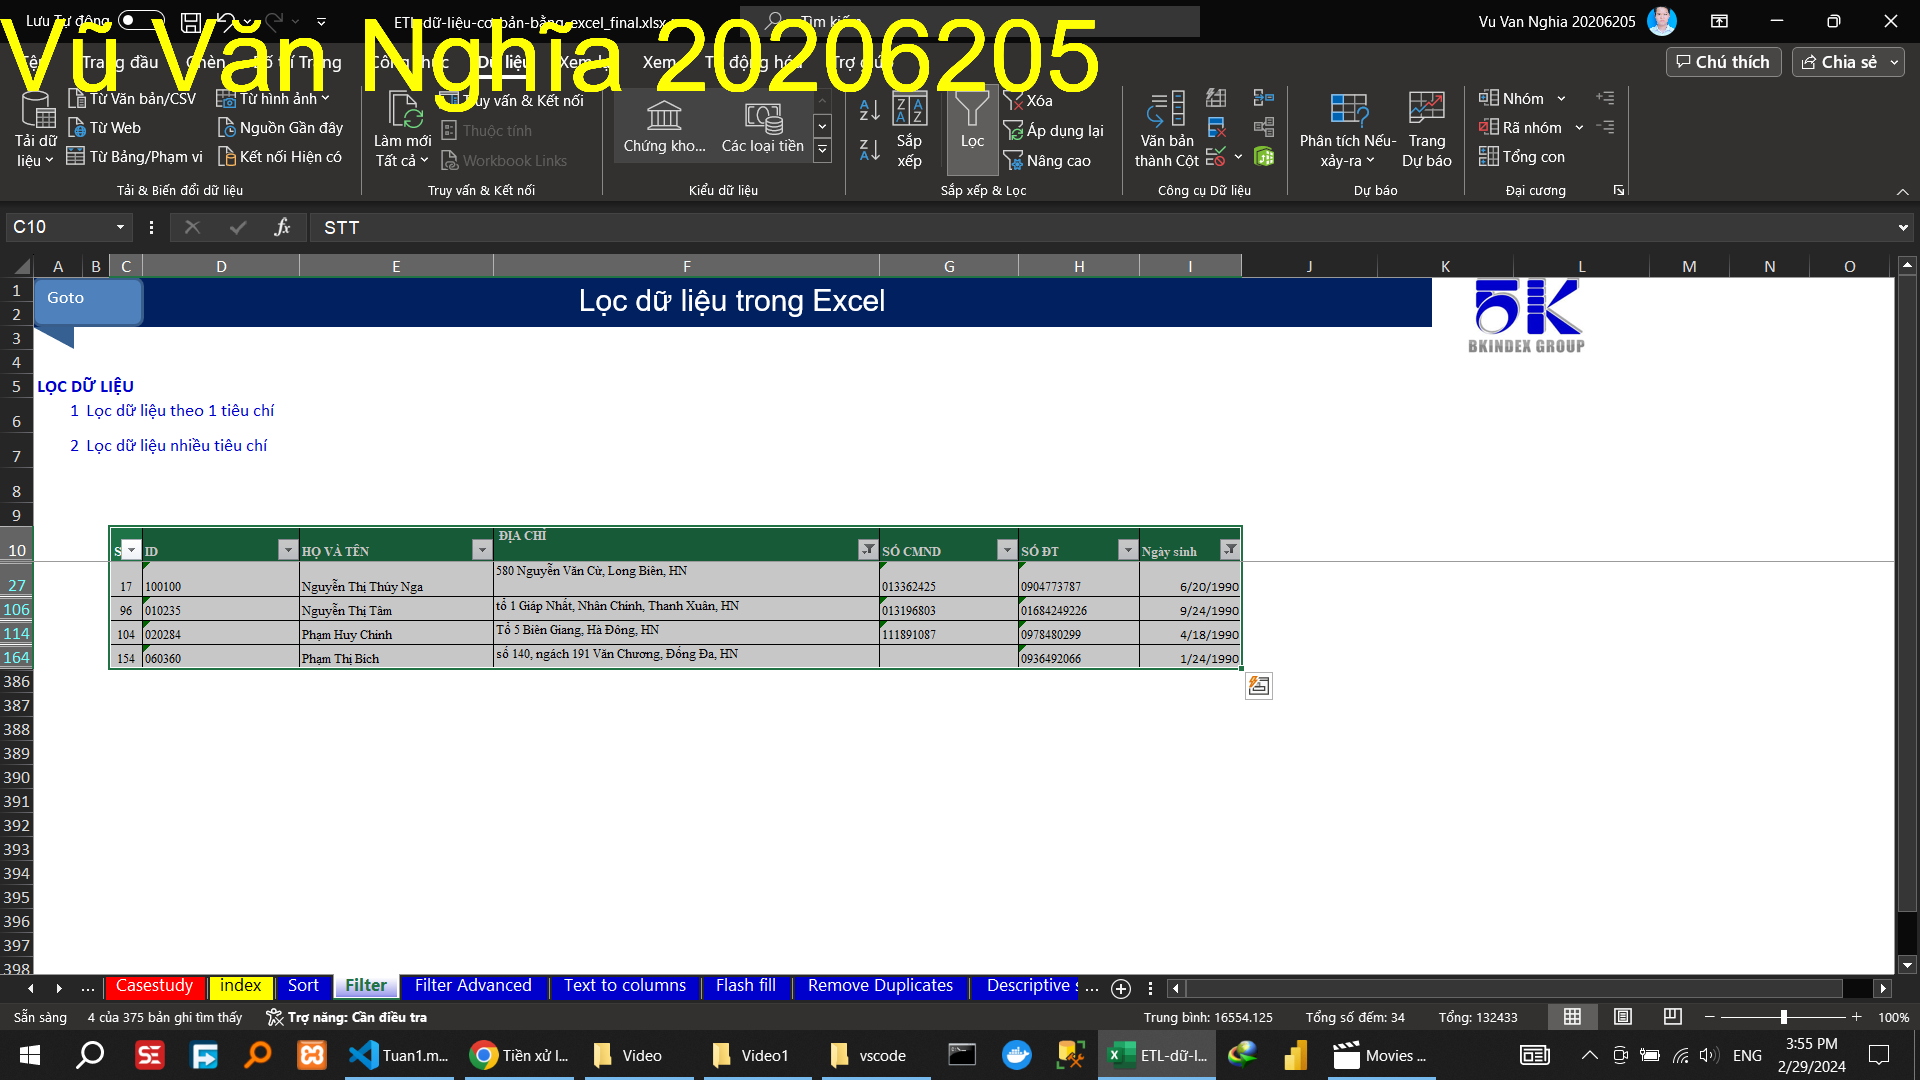
\includegraphics[scale = 0.15]{Video1/HuongDan/5.png}
%     \caption{Hướng dẫn lọc dữ liệu theo  nhiều tiêu chí địa chỉ và sinh năm 1990}
% \end{figure}




% \paragraph{Hướng dẫn lọc dữ liệu nâng cao}
% \subparagraph{Hướng dẫn lọc dữ liệu nâng cao theo 1 tiêu chí}
% \begin{figure}[h]
%     \centering
%     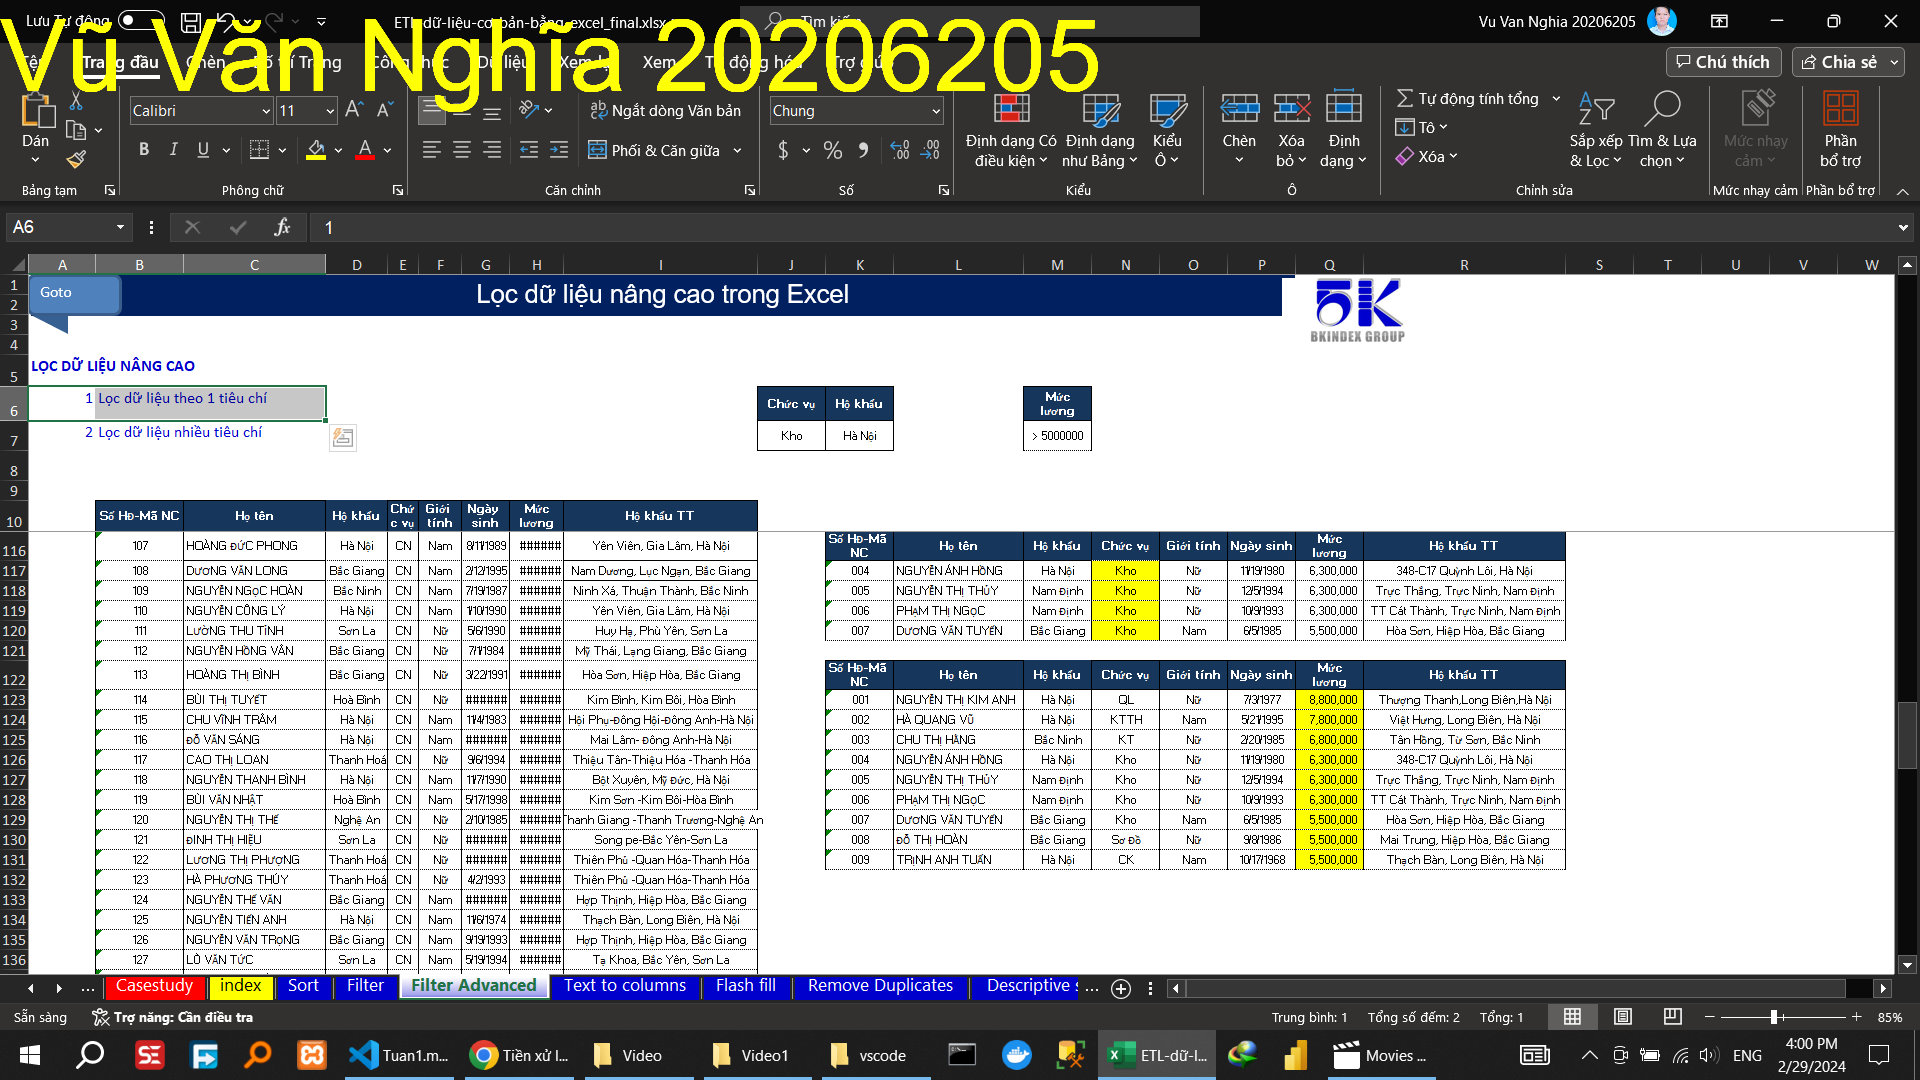
\includegraphics[scale = 0.15]{Video1/HuongDan/6.png}
%     \caption{Hướng dẫn lọc dữ liệu nâng cao theo 1 tiêu chí là chức vụ hoặc mức lương}
% \end{figure}
% \subparagraph{Hướng dẫn lọc dữ liệu nâng cao theo nhiều tiêu chí}
% \begin{figure}[h]
%     \centering
%     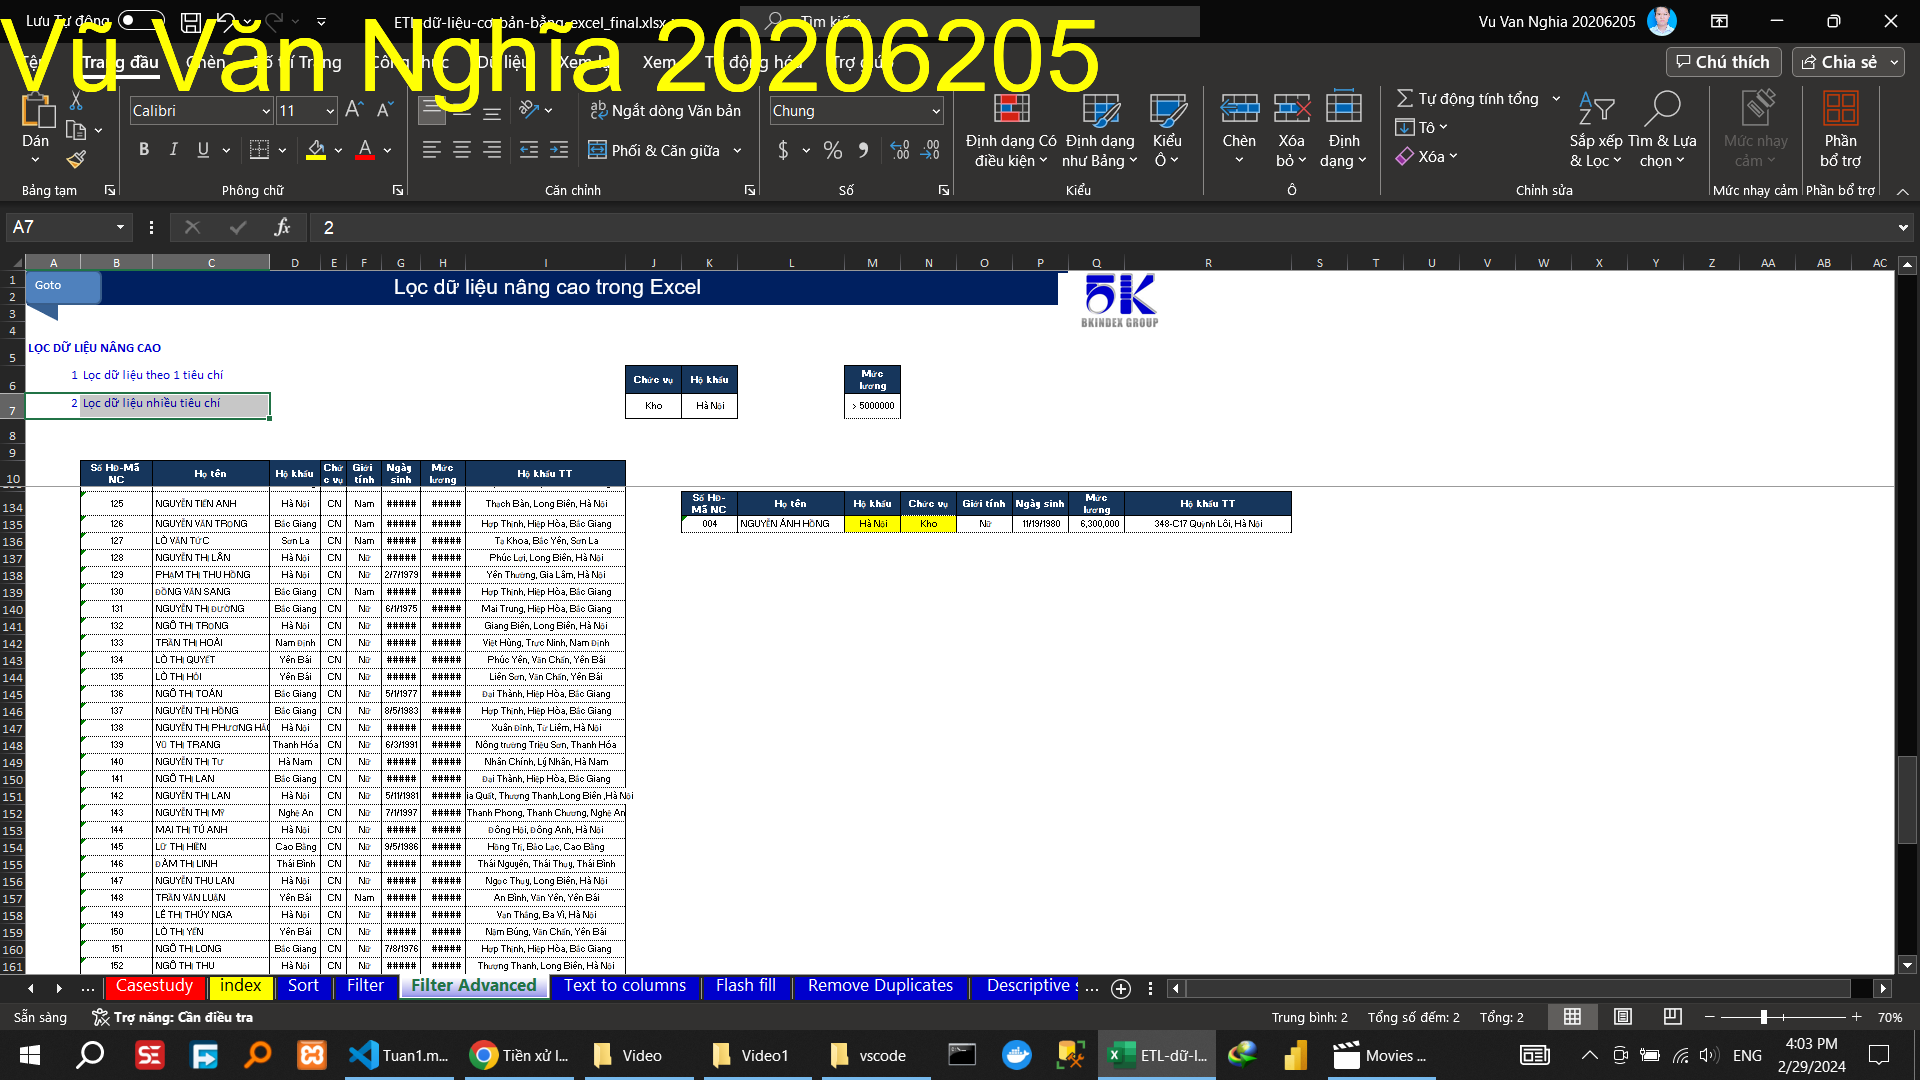
\includegraphics[scale = 0.15]{Video1/HuongDan/7.png}
%     \caption{Hướng dẫn lọc dữ liệu nâng cao theo  nhiều tiêu chí  chức vụ và hộ khẩu}
% \end{figure}



% \paragraph{Hướng dẫn tách cột văn bản thành nhiều cột}
% \subparagraph{Hướng dẫn  tách ngày tháng}
% \begin{figure}[h]
%     \centering
%     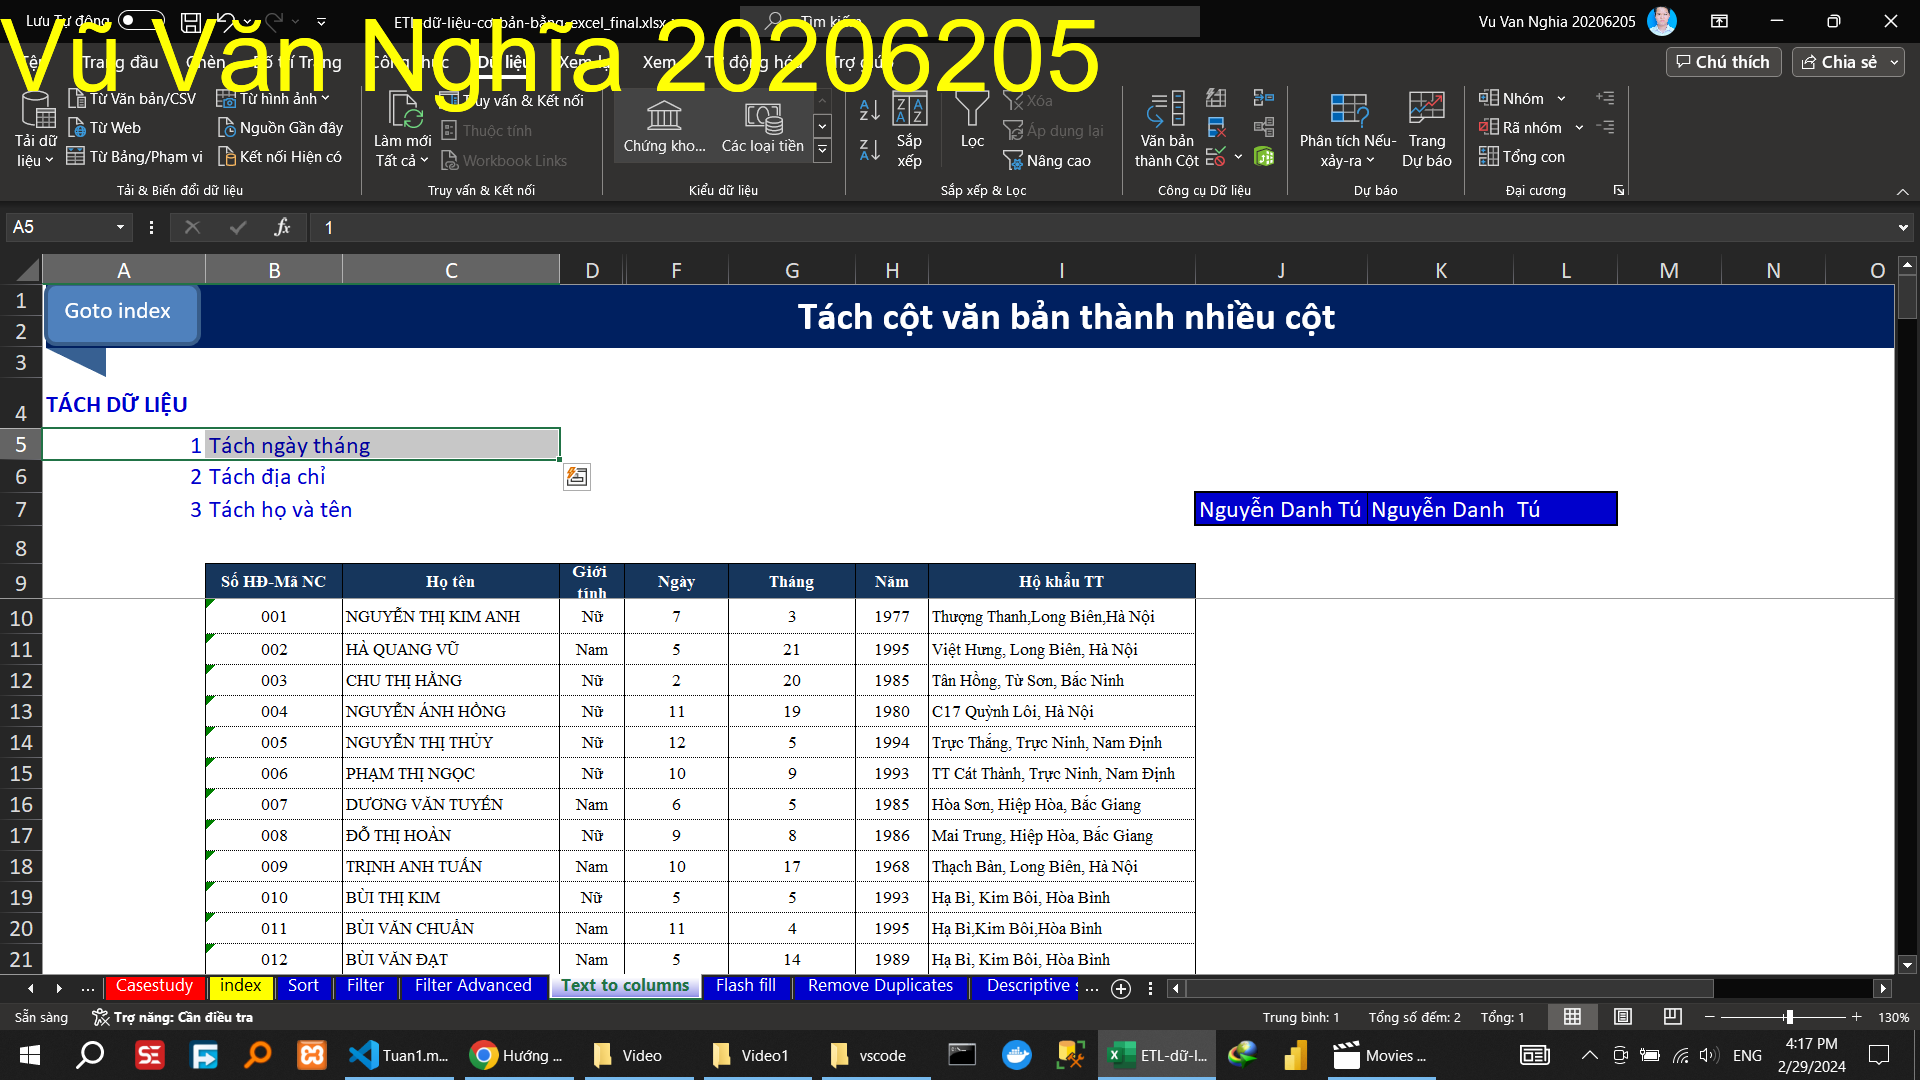
\includegraphics[scale = 0.15]{Video1/HuongDan/8.png}
%     \caption{Hướng dẫn  tách ngày tháng}
% \end{figure} 
% \subparagraph{Hướng dẫn  tách  địa chỉ}
% \begin{figure}[h]
%     \centering
%     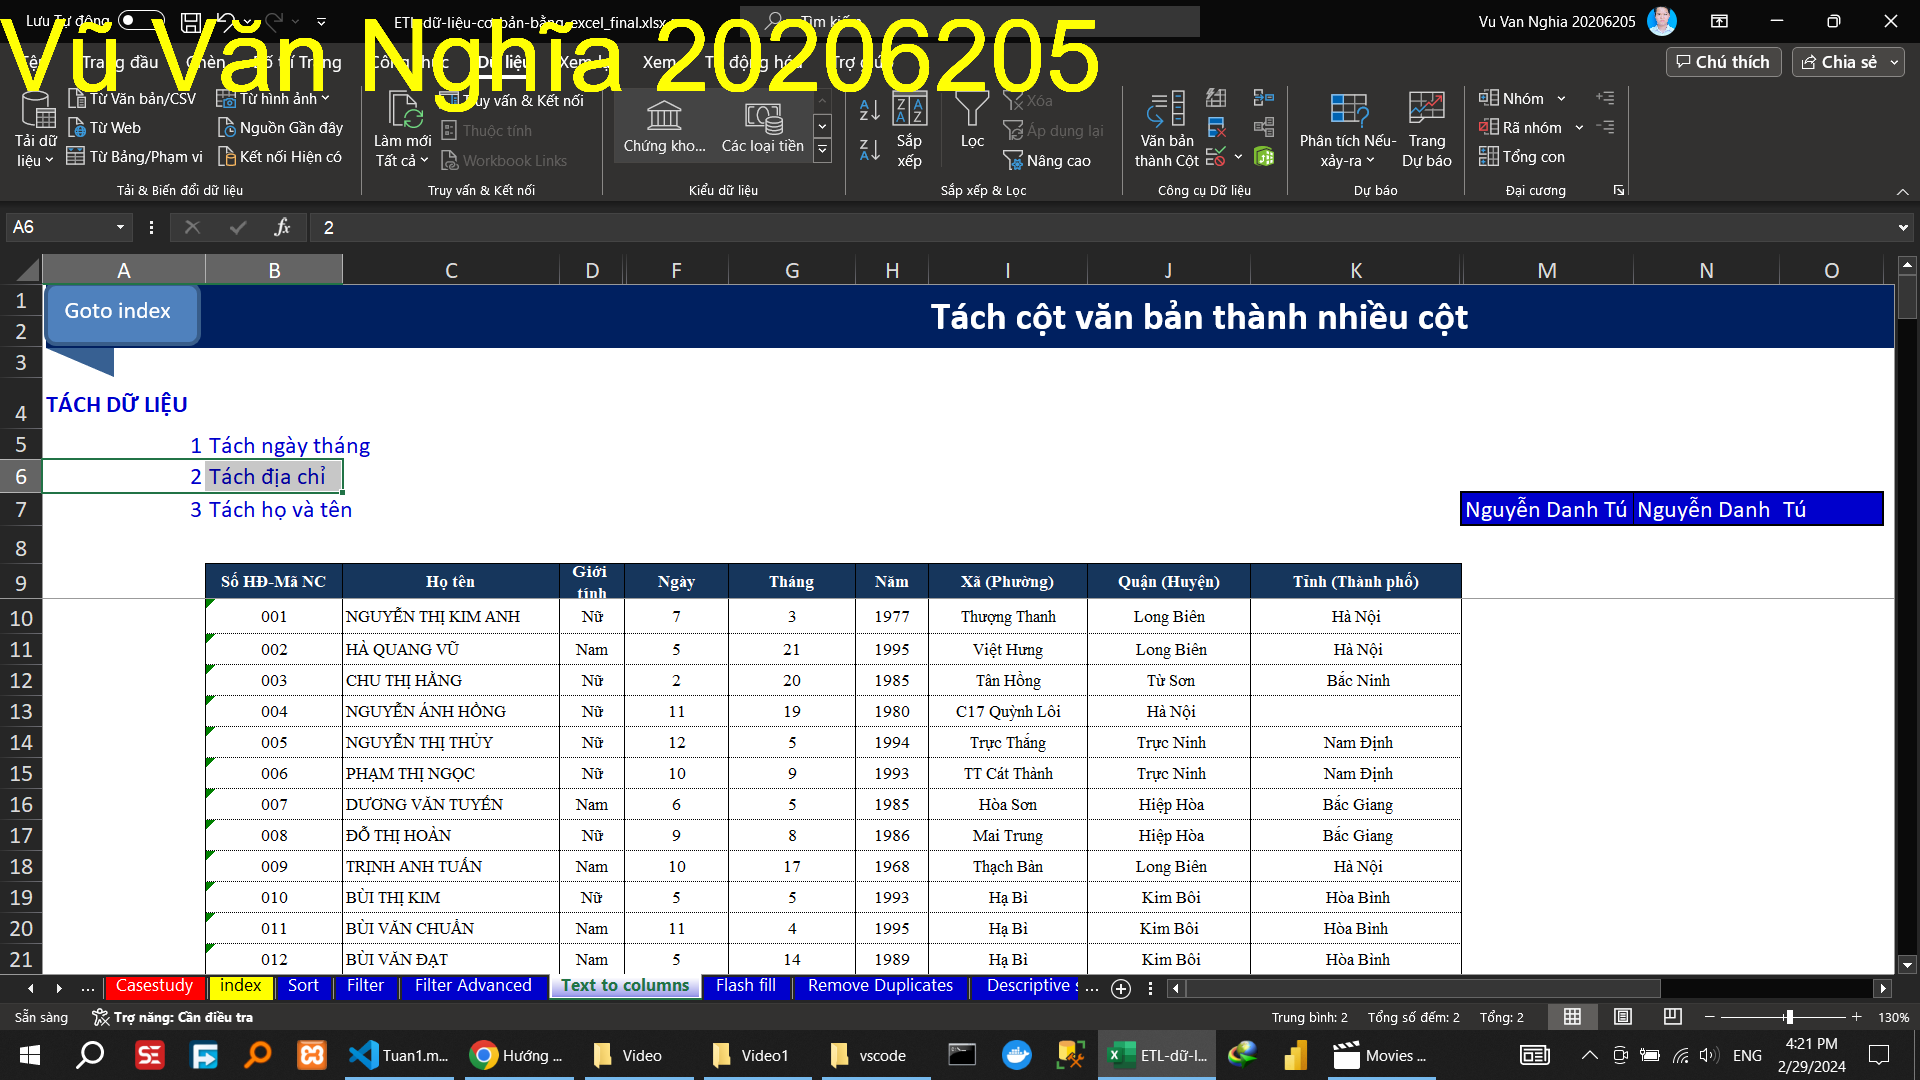
\includegraphics[scale = 0.15]{Video1/HuongDan/9.png}
%     \caption{Hướng dẫn  tách  địa chỉ}
% \end{figure} 
% \subparagraph{Hướng dẫn  tách  họ và tên}
% \begin{figure}[h]
%     \centering
%     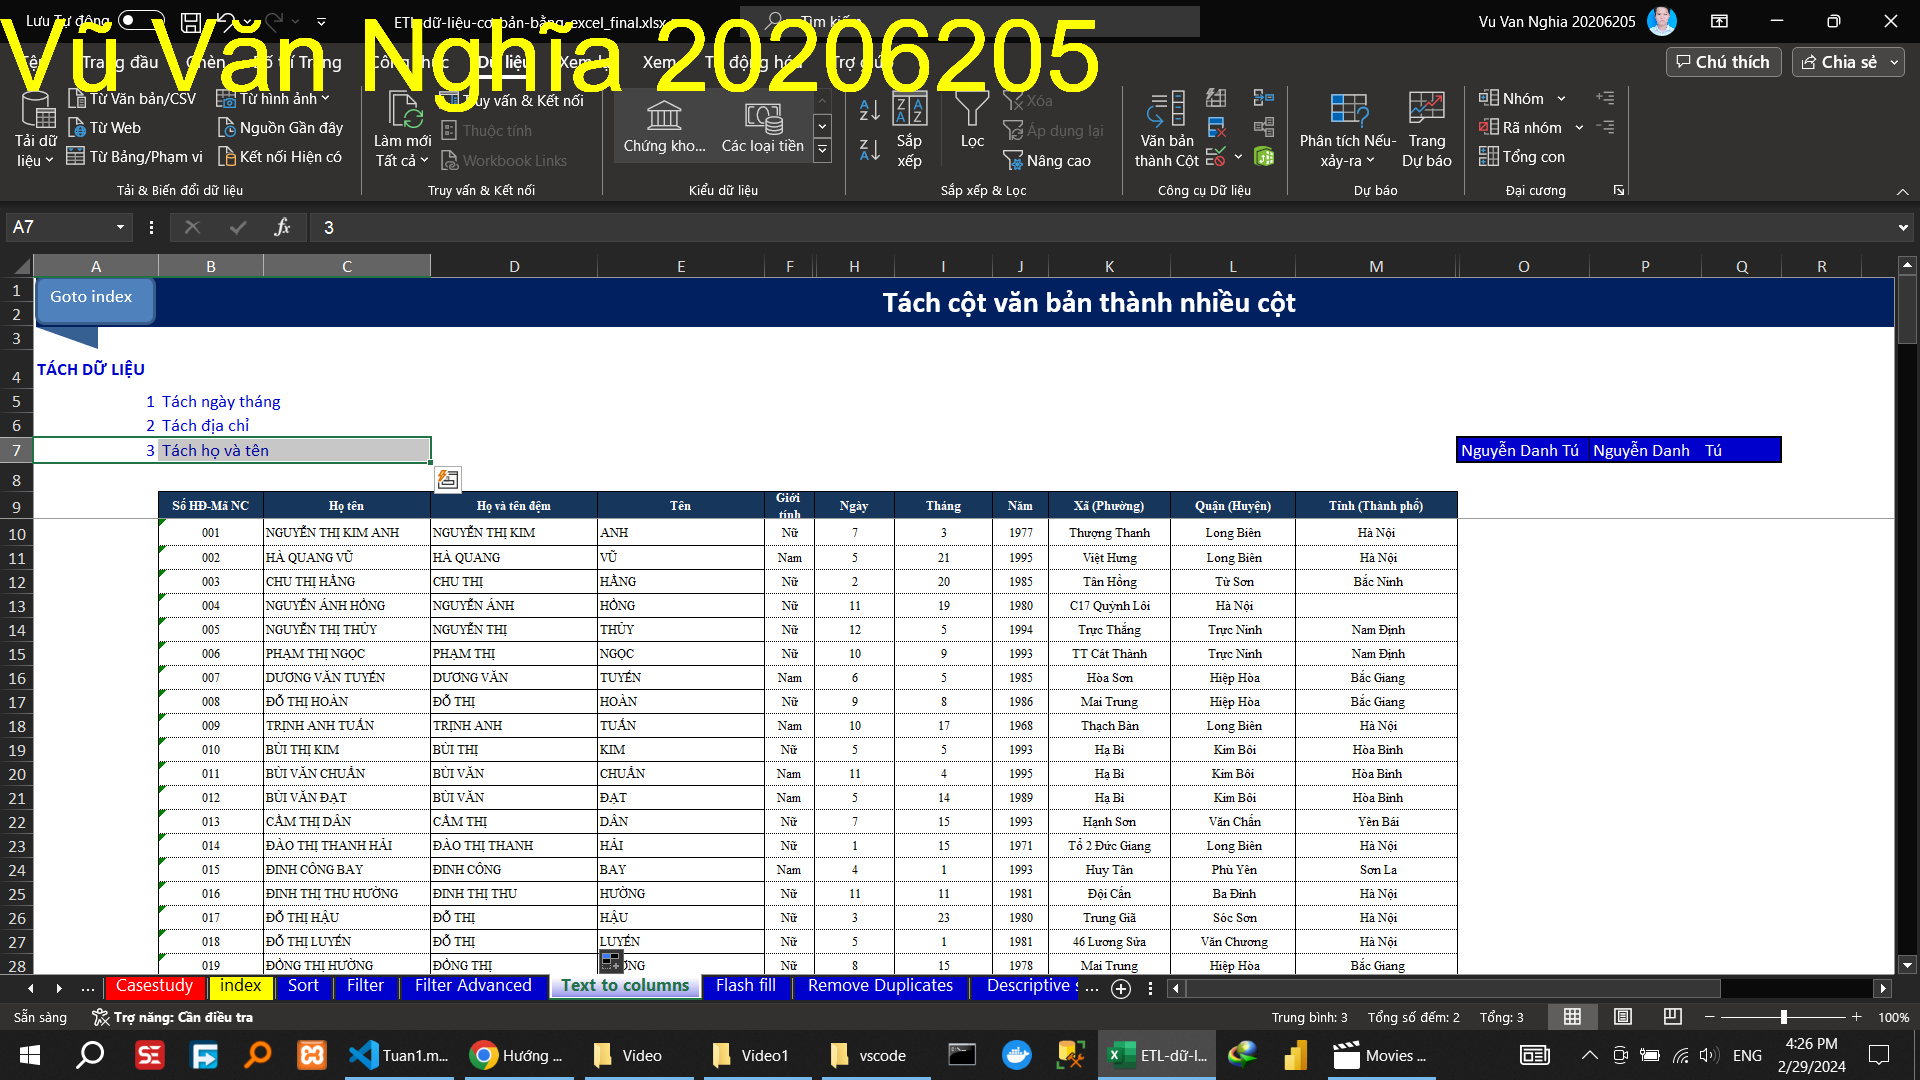
\includegraphics[scale = 0.15]{Video1/HuongDan/10.png}
%     \caption{Hướng dẫn  tách  họ và tên}
% \end{figure} 

   

% <!--  -->
% #### ĐIỀN DỮ LIỆU TỰ ĐỘNG

% ![xxxxxxxxxxxxxxxxxxxxxxxxxxx](HuongDan/11.png)

% #### XÓA DỮ LIỆU BỊ TRÙNG

% ![xxxxxxxxxxxxxxxxxxxxxxxxxxx](HuongDan/12.png)

% #### THỐNG KÊ MÔ TẢ

% ![xxxxxxxxxxxxxxxxxxxxxxxxxxx](HuongDan/13.png)

% ### Thực hành
  

% \paragraph{Hướng dẫn tách cột văn bản thành nhiều cột}
% \subparagraph{Hướng dẫn  tách ngày tháng}
% \begin{figure}[h]
%     \centering
%     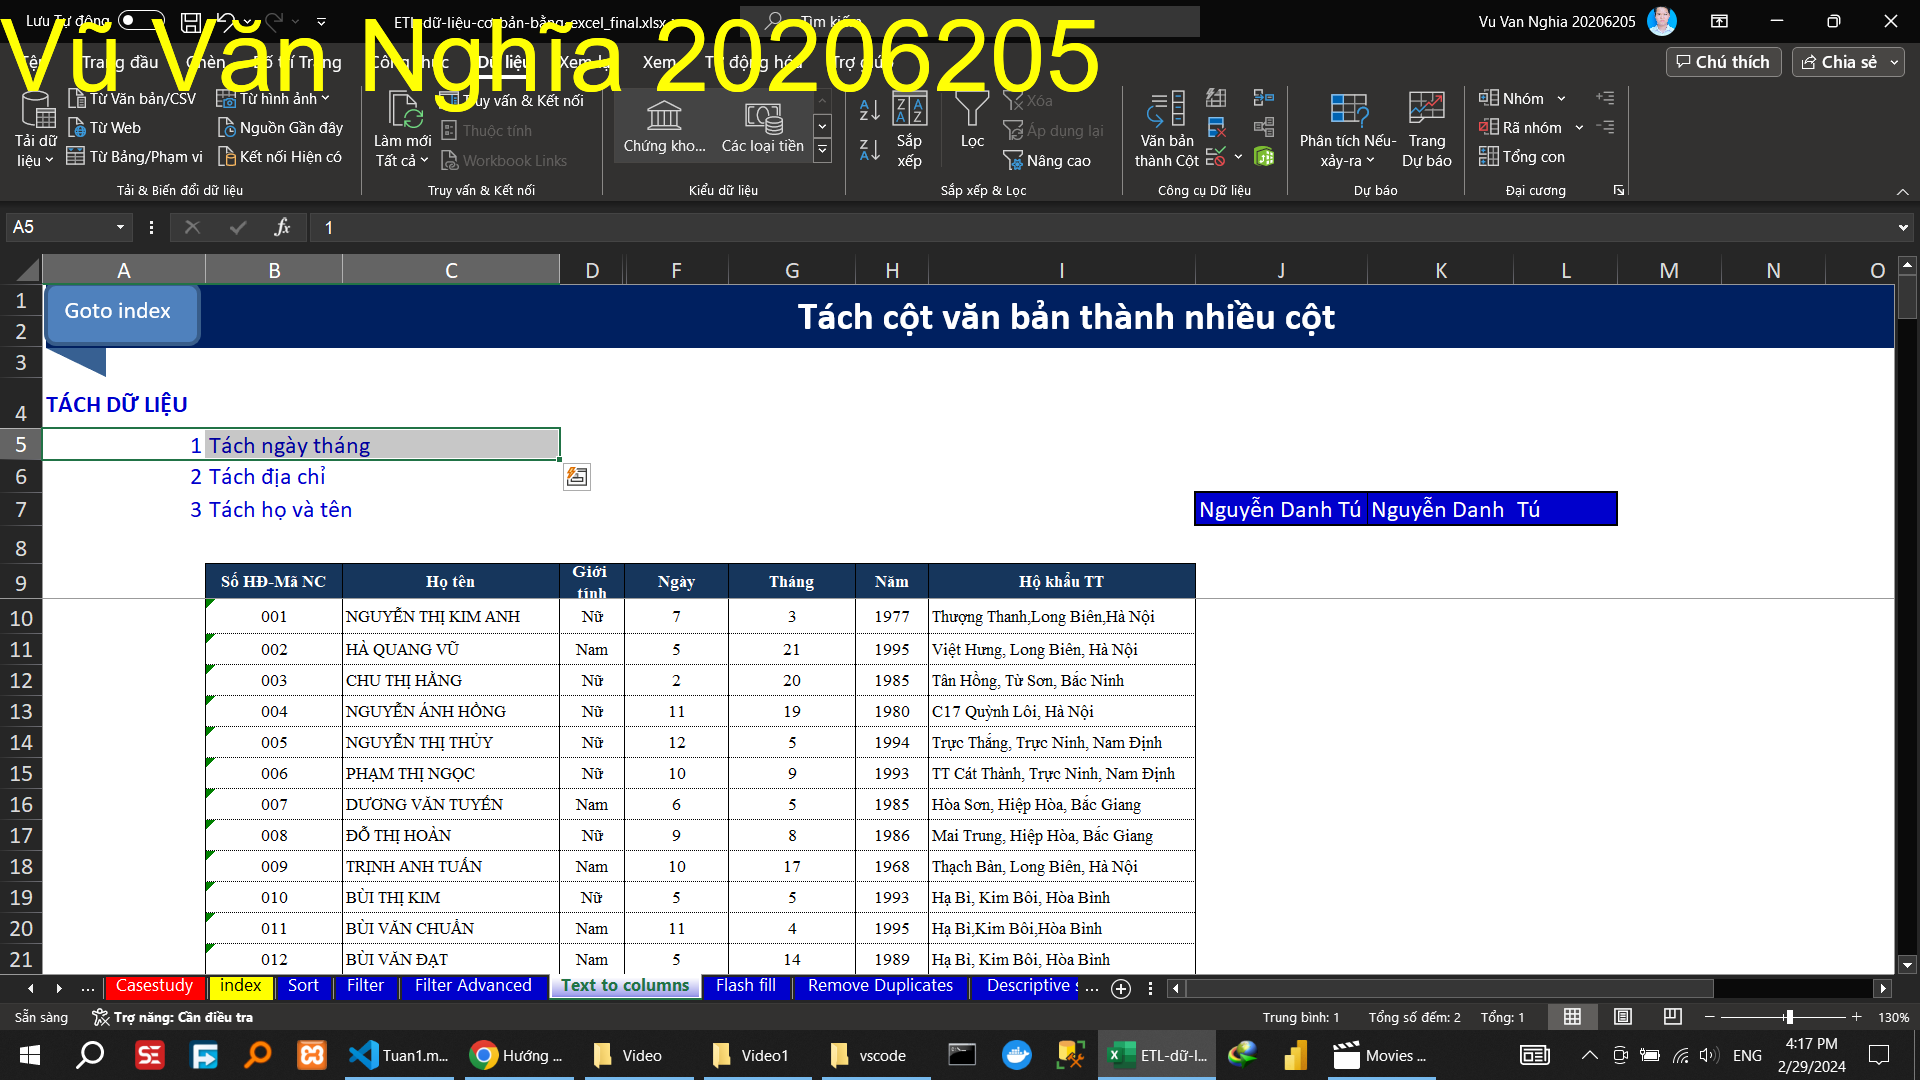
\includegraphics[scale = 0.15]{Video1/HuongDan/8.png}
%     \caption{Hướng dẫn  tách ngày tháng}
% \end{figure} 


\subsubsection{Thực hành}



\subsection{Video 2}
\subsubsection{Hướng dẫn}

\subsubsection{Thực hành}




\subsection{Video 3}
\subsubsection{Hướng dẫn}

\subsubsection{Thực hành}




\subsection{Video 4}
\subsubsection{Hướng dẫn}

\subsubsection{Thực hành}




\subsection{Video 5}
\subsubsection{Hướng dẫn}

\subsubsection{Thực hành}




\subsection{Video 6}
\subsubsection{Hướng dẫn}

\subsubsection{Thực hành}




\subsection{Video 7}
\subsubsection{Hướng dẫn}

\subsubsection{Thực hành}




\subsection{Video 8}
\subsubsection{Hướng dẫn}

\subsubsection{Thực hành}








%%%%%%%%%%%%%%%%%%%%%%%%%%%%%%%%%%%%%%%%%%%%%%%%%%%%%%%
\end{document}
%%%%%%%%%%%%%%%%%%%%%%%%%%%%%%%%%%%%%%%%%%%%%%%%%%%%%%%





\begin{figure}[h]
    \centering
    \includegraphics[width=0.5\textwidth]{example-image-a}
    \caption{Ví dụ về hình ảnh}
    \label{fig:example}
\end{figure}